\section{Performance Benchmarking}
\begin{frame}{\secname}{Disposition}
	Disposition
    \begin{itemize}
        \item Report Summary
        \item Concurrent Unit Management Benchmark
	\end{itemize}
\end{frame}

\subsection{Report Summary}\label{sec:authors}
\begin{frame}{\secname}{\subsecname}
	.NET Concurrency
	\begin{itemize}
		\item Lenient mapping to Async Workflows and \texttt{Task}s %up to speed?
		\item Sequential code faster in binary tree benchmarks
		\item Concurrent code faster with larger problem sizes:
		\begin{itemize}
			\item 11000 IL instructions in binary tree with no data dependency
			\item 44000 IL instructions in binary tree with data dependency
			\item Column sizes of 512 in matrix summation
		\end{itemize}
		\item Async Workflow concurrency is fragile
	\end{itemize}
\end{frame}

\begin{frame}{\secname}{\subsecname}
	Unity Performance
	\begin{itemize}
		\item Unity Technologies advices against functional coding style
		\begin{itemize}
			\item High order functions
			\item Closures
			\item Manipulate existing collections rather than mapping
		\end{itemize}
		\item Unit Management Benchmark
		\begin{itemize}
			\item F\# is marginally slower than C\# in Unity (5-7\%, \cite{maggiore2012formal,bolhuis2019gameplay})
			\item FRP system introduces per-\texttt{GameObject} overhead
		\end{itemize}
	\end{itemize}
\end{frame}

\begin{frame}{\secname}{\subsecname}
	Incorrect Code in Inverse Implementation of Unit Management Benchmark
	\begin{itemize}
		\item State machine has a list of units.
		\item When a unit collides with a shot, the unit is added to the list again.
		\item Many units =\textgreater\ many collisions =\textgreater\ performance degradation
	\end{itemize}
\end{frame}

\begin{frame}[fragile]{\secname}{\subsecname}
	Comparison of Incorrect and Correct Implementation
	\barChart*[12][\symbolic{Strategy,500,1000,1500,2000,2500}, width=\textwidth,height=.5\textheight][Average FPS][Number of Units]{Comparison of Correct and Incorrect implementation of Unit Management benchmark using the Mono runtime (higher is better).}{ai:benchmark}{
		\plotData{CSharp Correct}{\sequentialAverageData}
		\plotData{CSharp Incorrect}{\sequentialAverageData}
	}
\end{frame}

\subsection{Concurrent Unit Management Benchmark}

\begin{frame}{\secname}{\subsecname}
	Setup
	\begin{itemize}
		\item Examine if a concurrent implementation of inverse state machine is faster than sequential
		\item Bullets moved forward in a \texttt{Job}
		\item Each state's behaviour handled as a separate \texttt{Job}
		\item Moving between states sequentially
	\end{itemize}
\end{frame}

\begin{frame}{\secname}{\subsecname}
	Setup - Sequential
	\begin{figure}[h!]
        \centering
        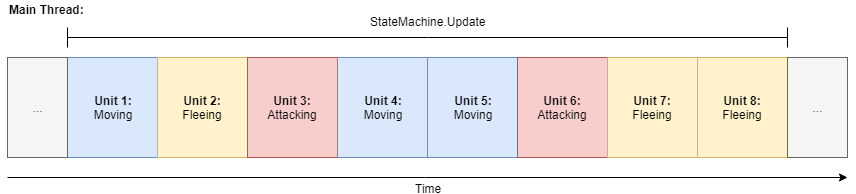
\includegraphics[width=.7\textwidth]{pictures/sequential.png}
        \caption{A model of sequential execution of inverse State Machine.}
    \end{figure}
\end{frame}

\begin{frame}{\secname}{\subsecname}
	Setup - Concurrent
	\begin{figure}[h!]
        \centering
        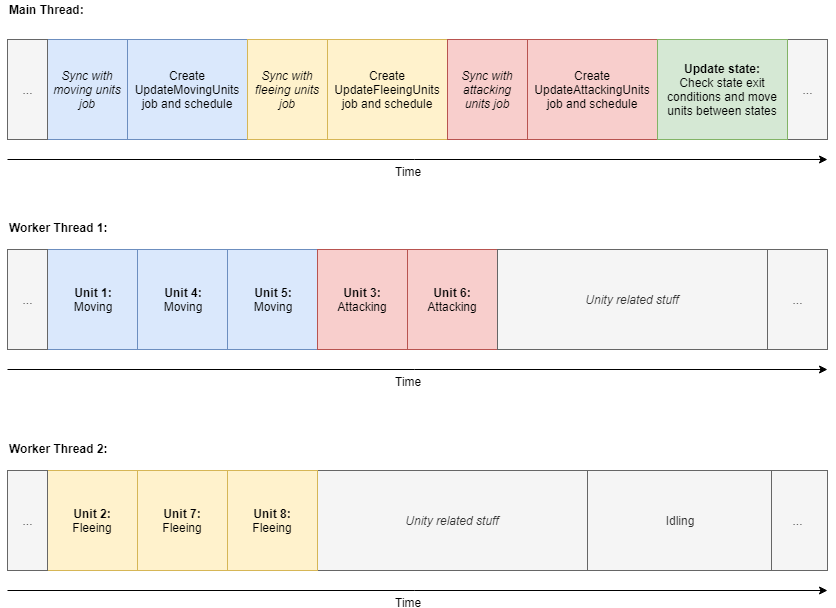
\includegraphics[width=.7\textwidth]{pictures/concurrent.png}
        \caption{A model of sequential execution of inverse State Machine.}
    \end{figure}
\end{frame}

\begin{frame}{\secname}{\subsecname}
	Experience with Unity C\# Job System
\end{frame}

\begin{frame}{\secname}{\subsecname}
	Results
\end{frame}

\begin{frame}{\secname}{\subsecname}
	Threats to Validity
\end{frame}
